\documentclass[letter, 12pt, oneside]{report}

\usepackage[T1]{fontenc}
\usepackage[utf8]{inputenc}
\usepackage[french, english]{babel}
\usepackage{textcomp}

\usepackage[a-1b]{pdfx}

\usepackage{newunicodechar}

\newunicodechar{⊃}{\ensuremath{\supset}}
\newunicodechar{⊂}{\ensuremath{\subset}}
\newunicodechar{∧}{\ensuremath{\land}}
\newunicodechar{∨}{\ensuremath{\lor}}
\newunicodechar{¬}{\ensuremath{\lnot}}
\newunicodechar{⊤}{\ensuremath{\top}}
\newunicodechar{⊥}{\ensuremath{\bot}}
\newunicodechar{→}{\ensuremath{\to}}
\newunicodechar{⊢}{\ensuremath{\vdash}}
\newunicodechar{⇒}{\ensuremath{\Rightarrow}}

\usepackage{tikz}
\usetikzlibrary{positioning}

\usepackage{inconsolata}

\usepackage{graphics}

\usepackage{xcolor}
\usepackage{xspace}

\usepackage{hyperref}

\usepackage{array}

\usepackage{datetime}
\newdateformat{monthyeardate}{\monthname[\THEMONTH], \THEYEAR}

\usepackage{geometry}

\usepackage{float}

\usepackage{multicol}

\usepackage{subcaption}

\usepackage{mathtools}

\usepackage{amsthm}

\newtheorem{theorem}{Theorem}
\newtheorem*{corollary}{Corollary}

\usepackage{amsmath}
\usepackage{amssymb}
\usepackage{stmaryrd}

\usepackage[printonlyreused, withpage]{acronym}

\usepackage{fancyvrb}
\fvset{listparameters=\setlength{\topsep}{0pt}\setlength{\partopsep}{0pt}}
\newcommand\verbpbf[1]{\textbf{#1}}
\newcommand\verbbf[1]{\textcolor[rgb]{0,0,1}{\textbf{#1}}}
\newcommand\verbrbf[1]{\textcolor[rgb]{1,0,0}{\textbf{#1}}}
\newcommand\verbprag[1]{\textcolor[rgb]{0.1,0.66,0.51}{#1}}
\newcommand\verbhole[1]{\textcolor[rgb]{1,0,0}{#1}}
\newcommand\verbcomment[1]{\textcolor[rgb]{0.6,0.6,0.6}{#1}}

\usepackage{minted}

\usepackage{needspace}

\usepackage{enumitem}

\usepackage{syntax}

\usepackage{vendor/proof}

\linespread{1.5}

\setlength{\leftmargin}{1in}
\setlength{\rightmargin}{1in}

\raggedbottom

\newcommand{\LF}{\ac{LF}\xspace}
\newcommand{\Beluga}{\textsc{Beluga}\xspace}
\newcommand{\Abella}{\textsc{Abella}\xspace}
\newcommand{\Agda}{\textsc{Agda}\xspace}
\newcommand{\Isabelle}{\textsc{Isabelle}\xspace}
\newcommand{\Isar}{\textsc{Isar}\xspace}
\newcommand{\HOL}{\textsc{HOL}\xspace}
\newcommand{\Coq}{\textsc{Coq}\xspace}
\newcommand{\CoqIDE}{\textsc{CoqIDE}\xspace}
\newcommand{\Lean}{\textsc{Lean}\xspace}
\newcommand{\Twelf}{\textsc{Twelf}\xspace}
\newcommand{\Hazel}{\textsc{Hazel}\xspace}
\newcommand{\Harpoon}{\textsc{Harpoon}\xspace}
\newcommand{\OCaml}{\textsc{OCaml}\xspace}
\newcommand{\SystemF}{\textsc{SystemF}\xspace}
\newcommand{\ocamlyacc}{\textsc{ocamlyacc}\xspace}
\newcommand{\ocamllex}{\textsc{ocamllex}\xspace}
\newcommand{\Commonmark}{\textsc{Commonmark}\xspace}
\newcommand{\Cpp}{\textsc{C++}\xspace}
\newcommand{\CamlpFour}{\textsc{Camlp4}\xspace}

\newcommand{\HTML}{\texttt{HTML}\xspace}
\newcommand{\XML}{\texttt{XML}\xspace}
\newcommand{\Markdown}{\texttt{Markdown}\xspace}

\newcommand{\set}[1]{\{#1\}}

\DeclarePairedDelimiter\ceil{\lceil}{\rceil}
\DeclarePairedDelimiter\floor{\lfloor}{\rfloor}
\DeclarePairedDelimiter\angled{\langle}{\rangle}
\DeclarePairedDelimiter\ucorner{\ulcorner}{\urcorner}

\makeatletter
\renewcommand\section{\@startsection {section}{1}{\z@}{-3.5ex \@plus -1ex \@minus -.2ex}{2.3ex \@plus.2ex}{\raggedright\normalfont\Large\bfseries}}
\makeatother

\usepackage{mdframed}
\mdfsetup{%
  frametitlebackgroundcolor=gray!20,
  frametitlerule=true,
  frametitlefont={\normalfont},
}


\begin{document}

\begin{titlepage}
\centering

\vspace*{0.5cm}

{\bfseries\LARGE Parsing, Lexical Scoping and Incremental Development for a Dependently-Typed Programming Language}

\vspace{1.8cm}

{\large Marc-Antoine Ouimet}

\vspace{2cm}

School of Computer Science

McGill University

Montreal, Quebec, Canada

\vspace{1.5cm}

\monthyeardate\today

\vspace{2cm}

A thesis submitted to McGill University in partial fulfilment\\
of the requirements of the degree of\\
Master of Science

\vfill

\raisebox{0.25ex}{\scalebox{0.8}{\textcopyright}}\ Marc-Antoine Ouimet, \the\year
\end{titlepage}


\clearpage

{\linespread{0.5}
\tableofcontents
}

\clearpage

\chapter*{Abstract}

\Beluga is a functional programming language and proof assistant for stating and mechanically proving theorems on systems specified in contextual \acs{LF}.
To facilitate the incremental development of proofs with commands and automation tactics, the \Harpoon interactive proof environment is subsequently implemented as a \acs{REPL} with structural editing features over \Beluga programs.
Of these features, the ability to seamlessly switch between holes in proofs is instrumental to proof development in top-down and out-of-order fashions, where proofs are postponed or partially completed.
However, this context-switching feature can cause soundness issues, resulting in the proof environment being invalid, and proof scripts translated to \Beluga programs failing semantic checks.
The root cause for these issues is due to architectural limitations in the implementation of \Beluga.

This thesis reports on technical challenges and solutions to soundly implementing the structural editing of proofs with navigation between proof holes, with a main focus on syntactic analysis and the early phases of semantic analysis.
Aspects of programming language syntax design are explored to support context-sensitive parsing of user-defined prefix, infix and postfix operators with a two-phase parser.
Then, name resolution for \Beluga is rectified with the implementation of a uniform referencing environment representation for indexing programs with separate contexts for different classes of variables.
Finally, the revised parser and name resolution phases are integrated into \Harpoon to ensure the state of identifiers in scope at any given proof hole is sound with respect to where the hole occurs.


\clearpage

% !TeX spellcheck = fr_CA

\chapter*{Résumé}
\vspace{-2em}

\Beluga est un langage de programmation fonctionnelle et un assistant de preuve pour spécifier des systèmes formels dans \acs{LF} contextuel, une extension du \acl{LF}, et prouver mécaniquement des théorèmes à propos d'eux au moyen de programmes récursifs.
Pour faciliter le développement incrémental de preuves, l'environnement interactif de preuve \Harpoon est implémenté en tant que \acl{REPL} avec des fonctionnalités d'édition structurelle de programmes écrits dans \Beluga.
À cause de limitations architecturales dans l'implémentation de \Beluga et \Harpoon, le développement de preuves vertical ou dans le désordre peuvent entraîner l'invalidation des états de preuve et la génération de programmes incorrects.

Cette thèse présente les défis techniques et les solutions à l'implémentation cohérente d'édition structurelle avec la navigation d'un endroit à l'autre dans des preuves incomplètes.
Un analyseur syntaxique contextuel est réalisé pour supporter la définition d'opérateurs préfixes, infixes et postfixes par l'utilisateur.
Ensuite, la résolution de noms pour \Beluga est rectifiée avec l'implémentation d'un environnement de référencement uniforme pour l'indexation de programmes définis par rapport à classes disjointes de variables.
Enfin, ces systèmes sont intégrés dans \Harpoon pour garantir que l'état des identifiants visibles à n'importe quel endroit dans une preuve incomplète est cohérent avec son emplacement.


\clearpage

\chapter*{Acknowledgements}
\addcontentsline{toc}{chapter}{Acknowledgements}

% TODO: Acknowledge Pientka's support throughout
% TODO: Acknowledge Johanna and Antoine's help revising the thesis
% TODO: Acknowledge Marie-Laurence for listening to my ramblings

% TODO: See https://www.mcgill.ca/gps/thesis/thesis-guidelines/preparation



\clearpage

\chapter*{Contributions}
\addcontentsline{toc}{chapter}{Contributions}

%This thesis presents original, unpublished work by the author Marc-Antoine~Ouimet under the supervision of professor Brigitte~Pientka.
Marc-Antoine~Ouimet contributed the entirety of this thesis, with feedback from peers and my supervisor as outlined in \hyperref[chapter:acknowledgments]{the acknowledgment page}.

Figure~\ref{figure:internal-syntax} is adapted from earlier works~\cite{nanevski2008contextual, germain2010implementation, cave2013first, ferreira2013compiling} on \Beluga.


\clearpage

\begin{figure}
\begin{tabular}{rrll}
\LF kinds & $ K $ & $ \Coloneqq $ & $ \mathsf{type} \mid \Pi x {:} A. K \mid A \to K $\\
\LF types & $ A, B $ & $ \Coloneqq $ & $ \mathbf{a} \mid A \to B \mid A \; M_1 \; M_2 \; \dots \; M_n $\\
\LF terms & $ M, N $ & $ \Coloneqq $ & $ \mathbf{c} \mid x \mid \lambda x {:} A. M \mid M \; N_1 \; N_2 \; \dots \; N_n \mid M : A $
\end{tabular}

\caption{External syntax definition.}
\end{figure}

\chapter{Introduction}\label{chapter:introduction}

% What is mechanized meta-theory?

% What are dependently-typed programming languages?

% What is Beluga? What is HOAS? What is contextual modal type theory?

\Beluga~\cite{pientka2010beluga} is a dependently-typed programming language for specifying and proving properties about formal systems using contextual modal type theory~\cite{nanevski2008contextual}.
It leverages the \acf{LF}~\cite{harper1993framework}, extended with explicit contexts, contextual objects and substitutions~\cite{DBLP:journals/corr/abs-1009-2789, cave2013first}, which allow for logic reasoning involving open terms.
Using \ac{HOAS}~\cite{pfenning1988higher}, elegant and succinct datatype definitions can be made in \LF to subsequently prove theorems pertaining to programming languages and $ \lambda $-calculi.
These proofs are encoded as programs written in a functional style, together with checkers to ensure they always terminate and cover all possible cases~\cite{dunfield2009, inductivebeluga}.
Propositions then correspond to types, and well-founded reasoning by induction corresponds to recursion with totality and coverage checking.
With this framework, \Beluga has notably been used to mechanically verify proofs for the type safety of \SystemF~\cite{poplmarkreloaded}, termination of weak-head normalization for the simply-typed lambda calculus~\cite{cave2013first}, and type preservation for a session-typed system based on classical linear logic~\cite{sano2023}.
Extensions to \Beluga have facilitated the development of proofs by providing interactive tools for manipulating and constructing proof terms.

% How does one specify a formal system using Beluga?

% What are interactive theorem provers?

Interactive theorem proving is the computer-assisted process of finding valid proofs for propositions in a logic system.
Proof assistants have been implemented and successfully leveraged to prove fundamentals of mathematics and type theories.
\Agda~\cite{clffolp, norell2007towards, agda2023}, \Coq~\cite{Coq, bertot2013interactive}, \Isabelle~\cite{nipkow2002isabelle} and \Lean~\cite{lean4} are among the most prevalent proof assistants used in the formalization of programming languages.
Functionalities of typical interactive theorem provers range from \acp{REPL} allowing for structural editing and code inspection to automated proof search to generate valid programs.

% What is Harpoon?

\Harpoon~\cite{errington2021harpoon} is a command-line frontend to \Beluga for proving theorems interactively.
It provides a proof development workflow closer to proofs on paper, with built-in commands replicating proof techniques such as case analyses and appeals to induction hypotheses.
Additional administrative commands are supported to navigate through the history of input commands, and to checkout different holes in proofs declared elsewhere in \Beluga signatures.
Upon closing interactive sessions, \Harpoon produces verbose yet simple tree-shaped proof scripts which can be translated into well-formed \Beluga programs.
\Harpoon's design is largely inspired by \Coq's interactive proof mode using tactics~\cite{delahaye2000tactic} to solve unproven goals.
Crucially, \Harpoon is a system integrated into \Beluga's core functionalities in such a way that the overall proof state does not have to be reconstructed from scratch on every command, which is akin to structural editing.

% What is structured editing?

Structural (or projectional) editing in programming language tooling is the functionality of a software editor that allows the user to manipulate \acp{AST} directly.
This is in contrast with plain text editors in which users may only edit textual representations of their programs, that then subsequently require parsing to be interpreted.
The \Hazel~\cite{omar2017hazelnut, omar2019live} functional programming environment is a notable example of a structural editor in the functional programming community for its ability to dynamically provide type information as the user writes programs with holes.
This is achieved using carefully designed semantics of moving a text-editing cursor in the concrete syntax and mapping its location to a node in the parsed \ac{AST}.
When it comes to theorem provers, one example of structured editing is the \CoqIDE~\cite{Coq}, which leverages the \Coq \XML protocol and a state transaction system to interact with the proof system's kernel by way of messages.
This is not too dissimilar to what is done with implementations of the language server protocol to provide advanced editing functionalities for programming languages.
In essence, the main objectives for implementing structural editing are to enable and assist in the incremental development of programs.
This is in contrast with incremental compilation, which focuses on recompiling minimal sets of programs when they are affected by changes to the source code, which is achieved using dependency analysis and careful handling of cache invalidations.

% What are typical edit actions in programming languages?

Structural editors define sets of edit actions the user may execute at given points in their editing session.
Typical edit actions include navigating the \ac{AST} being modified, or constructing new nodes using either a graphical interface or a textual language.
These actions are then reflected in the editor state in a predictable way, such that the edited program does not need to be reparsed from scratch.
Having a greater control over how a program is edited is also used to prevent or signal edit actions that can invalidate a program.
This can be as simple as signalling type errors on-the-fly, or in the case of theorem provers, to reject unsound operations like invalid appeals to induction hypotheses.

% What are edit actions required by Beluga and Harpoon?

Although \Beluga's interactive mode and \Harpoon are \acp{REPL} as opposed to full-fledged structural editors, they do share some functional requirements.
Indeed, like in \Isabelle, \Hazel and \Coq, users of \Beluga and \Harpoon postpone the completion of programs or proof scripts by inserting holes in them.
These holes stand for missing expressions, and they are later filled in with the help of a proof assistant that provides typing information for the identifiers in scope for each hole.
As such, both \acp{REPL} and structural editors are required to construct and update an editor state as the user performs edit actions.

% In general, what are challenges to implementing edit actions?

Edit actions in \Beluga and \Harpoon include navigating between holes in programs and proof scripts respectively, as well as displaying type information for expressions, and performing case analyses on meta-level and computation-level objects identified by (meta-)variables.
These actions require surgical manipulation of the editor state to ensure soundness of the \ac{AST} being edited is preserved, as well as to prevent the undesirable propagation of information like typing constraints in unrelated edit locations.

% In Beluga and Harpoon specifically, what are the challenges to implementing edit actions?

Historically, \Beluga was not implemented with the mindset of supporting the level of interactivity that \Harpoon purports to have.
Indeed, as is the case with prototype implementations of programming languages, \Beluga's early development focused on implementing a parser for its concrete syntax and a type-checker for its type theory.
The software architectural pattern that arose from this implementation was the pipeline pattern, in which the data processing of programs from its textual to its \ac{AST} representation is handled in single-responsibility phases that sequentially augment and refine the data for later use.
Specifically with respect to \Beluga, these phases have evolved to include implicit argument reconstruction, the translation from a named to a nameless representation of binders using de Bruijn indices, term normalization, type-checking, and totality-checking.
What transpires from this design is a unilateral flow of information from the concrete syntax to the internal representation of programs in \Beluga.
Early optimizations were put in place to maximize the performance of this processing pipeline.
In particular, a single global mutable representation of the \Beluga program being processed was implemented to provide information to later processing phases in a feedforward fashion.
This simplified the implementation of new features since globally accessible data does not need intricate data routing procedures like dependency injection.
This design was sound only under the assumption that the necessary information for processing \Beluga signatures would flow in only one direction.
Unfortunately, the introduction of \Beluga's interactive mode and subsequently \Harpoon inadvertently broke that assumption.
Indeed, soundness issues have arose with regards to features and processes of the two systems that require inspecting only a subset of a signature, and as such using referencing environments built out of order.
This issue of locality in references has further been shown to deteriorate the performance of \Beluga's logic programming engine used to automate proof search.

% What is the proposed approach to supporting edit actions in Beluga and Harpoon?

%In particular, we present an explicitly stateful algorithm for the parsing, disambiguation and indexing of \Beluga programs to ensure correct name resolutions across editing states.
%This fixed the soundness issue for \Harpoon proof sessions whereby constants declared after the proof hole would be in scope and shadow earlier declarations.
%The revised approach to name resolution allowed for consistent namespacing of constants to be implemented.
%Additionally, the \Beluga feature of fixity pragmas for defining prefix, infix or postfix notations for \LF-level constants was expanded upon to also work with computation-level constants.
%Using the proposed specification for \Beluga and \Harpoon's grammars, the generation of \HTML pages corresponding to signatures was restored, with a new and improved pretty-printing algorithm of the concrete syntax.
%Overall, the changes have improved the maintainability, resiliency and stability of the affected modules, and have proposed better architectural design patterns that may be applied to the rest of the implementation.

This thesis reports on improvements made to the implementation \Beluga and \Harpoon to address some of the soundness issues in interactive proof development in these two systems.
Overall, the changes listed below have improved the maintainability, resiliency and stability of the affected modules.
Better architectural software design patterns have been put in place, and these may be expanded upon in future iterations on the later phases of semantic analysis.
The specific contributions of this work are:
\begin{enumerate}
\item
A complete and formal specification of \Beluga and \Harpoon's grammars for parsing.
\item
A robust implementation of a context-free parser for \Beluga and \Harpoon, along with a new context-sensitive disambiguation phase to rectify and expand existing features.
Most notably, the \Beluga feature of fixity pragmas for defining prefix, infix or postfix notations for \LF-level constants is reworked to also support computation-level constants.
\item
A uniform name resolution algorithm to improve the clarity of \Beluga programs, implement namespaces, and to support sound incremental proof development.
This fixed soundness issues for \Harpoon having to do with its feature of navigation between holes in proofs anywhere in a \Beluga signature.
\item
An improved and context-aware pretty-printing algorithms for formatting \Beluga programs in external \ac{AST} representation, and for generating corresponding \HTML pages.
\end{enumerate}


\chapter{Background}

\section{The \Beluga Language}

In \Beluga, theorems are encoded using contextual \LF, its index language, and proofs are encoded as programs.
Logic propositions are represented as \LF type families with term-level constants parameterized by $\beta$-normal $\eta$-long \LF terms to construct witnesses for these propositions~\cite{nanevski2008contextual, foundation2008pientka, DBLP:journals/corr/abs-1009-2789}.
To facilitate the implementation of semantic analysis, and because \LF kinds, types and terms are strongly normalizing~\cite{harper1993framework}, they are required to be encoded in normal form by the user.
\Beluga extends \LF to support explicit contexts and substitutions, which enables mechanized reasoning with respect to assumptions, like in proofs on paper~\cite{pientka2010programming}.
This means that terms containing free variables can be manipulated and reasoned about explicitly in \Beluga.

A signature in \Beluga is the list of all the toplevel constant declarations in a mechanization.
This includes the aforementioned \LF type-level and term-level constant declarations, but also includes inductive and coinductive type declarations at the computation-level, with their associated constructors and destructors respectively, and computation-level programs.
\Harpoon provides an alternative to specifying proofs as programs in the form of a proof script comprised of tactics and their effects on the meta-level and computation-level contexts for variables.
A complete specification of signature-level declarations is provided in section~\ref{section:syntax-signature} as part of grammars for parsing.

% TODO:

Let $x$ and $c$ range over computation-level variables and constants respectively, $X$ range over meta-object variables, $\psi$ over context variables and $g$ over context schemas.
Figure~\ref{figure:internal-syntax} then provides an overview of \Beluga's core language.
\LF kinds classify \LF types, which classify \LF terms.
Likewise, computation-level kinds classify computation-level types, which classify computation-level expressions.
\LF terms are broken down into normal and neutral terms, along with heads and spines, to syntactically enforce canonical forms.
The notation $A \to K$ is used for the \LF kind $\Pi x{:}A. K$ when $x$ does not appear free in $K$.
The notation $A \to B$ is defined analogously for \LF types.
Since \Beluga's type system is bidirectional, the syntax of computation-level expressions is split into those for which a type can be inferred (type-synthesizing expressions), and those that can be checked against a type (type-checkable expressions).
Meta-objects, classified by meta-types, can be embedded in the computation-level by way of boxes that simultaneously bind all variables from \LF contexts.

% What's the point of meta-level constructs?

% TODO: Go over some topics from Programming Inductive Proofs - A New Approach Based on Contextual Types, namely type reconstruction, totality

\begin{figure}
\begin{subfigure}{\linewidth}
\begin{tabular}{p{5.5cm} >{\raggedleft}p{1cm} r l}
\LF kinds & $K$ & $\Coloneqq$ & $\Pi x{:}A. K \mid \mathbf{type}$\\
\LF types & $A, B$ & $\Coloneqq$ & $\Pi x{:}A. B \mid P$\\
Atomic \LF types & $P$ & $\Coloneqq$ & $a \cdot S$\\
\LF normal terms & $M$ & $\Coloneqq$ & $R \mid \lambda x. M$\\
\LF neutral terms & $R$ & $\Coloneqq$ & $H \cdot S \mid u[\sigma]$\\
\LF heads & $H$ & $\Coloneqq$ & $x \mid c \mid p[\sigma]$\\
\LF spines & $S$ & $\Coloneqq$ & $\cdot \mid M\ S$\\
Substitutions & $\sigma$ & $\Coloneqq$ & $\cdot \mid \mathsf{id}_\psi \mid \sigma, M \mid \mathsf{id}_\psi[\rho]$\\
Substitution closures & $\rho$ & $\Coloneqq$ & $s[\sigma]$\\
Contexts & $\Psi$ & $\Coloneqq$ & $\cdot \mid \psi \mid \Psi, x : A$\\
\end{tabular}
\caption{Internal syntax of contextual \LF in \Beluga.}
\end{subfigure}
\par\bigskip
\begin{subfigure}{\linewidth}
\begin{tabular}{p{5.5cm} >{\raggedleft}p{1cm} r l}
Meta-types & $U$ & $\Coloneqq$ & $\cdots \mid g \mid (\Psi \vdash A) \mid (\Psi \vdash \Psi)$\\
Meta-objects & $C$ & $\Coloneqq$ & $\cdots \mid \Psi \mid (\Psi \vdash M) \mid (\Psi \vdash \sigma)$
\end{tabular}
\caption{Internal syntax of \Beluga's meta level (excerpt).}
\end{subfigure}
\par\bigskip
\begin{subfigure}{\linewidth}
\begin{tabular}{p{5.5cm} >{\raggedleft}p{1cm} r l}
Computation-level kinds & $\kappa$ & $\Coloneqq$ & $[U] \to \kappa \mid \Pi X{:}U. \kappa \mid \mathbf{ctype}$\\
Computation-level types & $\tau$ & $\Coloneqq$ & $\cdots \mid c \mid \tau_1 \to \tau_2 \mid \Pi X{:}U. \tau \mid [U] \mid \tau\ [C]$\\
Type-checkable expressions & $e$ & $\Coloneqq$ & $\cdots \mid i \mid [C] \mid \mathbf{fn}\ x \Rightarrow e \mid \mathbf{mlam}\ X \Rightarrow e$ \\
& & $|$ & $\mathbf{let}\ x = i\ \mathbf{in}\ e \mid \mathbf{case}\ i\ \mathbf{of}\ \overrightarrow{p \Rightarrow e}$\\
Type-synthesizing expressions & $i$ & $\Coloneqq$ & $\cdots \mid x \mid c \mid i \ e \mid e : \tau$
\end{tabular}
\caption{Internal syntax of \Beluga's computation level (excerpt).}
\end{subfigure}
\caption[Excerpt of \Beluga's internal syntax]{%
Excerpt of \Beluga's internal syntax~\cite{nanevski2008contextual, germain2010implementation, cave2013first, ferreira2013compiling} used in discussions about its theory.
}
\label{figure:internal-syntax}
\end{figure}

\clearpage

To illustrate how \Beluga is leveraged to mechanically prove properties about formal systems, consider the following running example adapted from \cite{felty2010reasoning} where it is shown that algorithmic equality for the untyped $\lambda$-calculus is reflexive.

{\footnotesize
\begin{mdframed}[frametitle={$\boxed{\Gamma \vdash \Term{M}}$ : the term $M$ is well-formed in context $\Gamma$}]
\begin{equation}
\infer{\Gamma \vdash \Term{x}}{x \in \Gamma}
\end{equation}
\begin{equation}
\infer{\Gamma \vdash \Term{\lambda x. M}}{\Gamma, x : \mathsf{term} \vdash \Term{M}}
\end{equation}
\begin{equation}
\infer{\Gamma \vdash \Term{M\ N}}{\Gamma \vdash \Term{M} & \Gamma \vdash \Term{N}}
\end{equation}
\begin{equation}
\infer{\Gamma \vdash \Term{\Unit}}{}
\end{equation}
\end{mdframed}

\begin{mdframed}[frametitle={$\boxed{\Gamma \vdash M \equiv N}$ : the term $M$ is algorithmically equal to $N$ in context $\Gamma$}]
\begin{equation}
\infer[\equiv\text{-lam}]{\Gamma \vdash \lambda x. M \equiv \lambda x. N}{\Gamma, x : \mathsf{term}, e : x \equiv x \vdash M\ x \equiv N\ x}
\end{equation}
\begin{equation}
\infer[\equiv\text{-app}]{\Gamma \vdash M_1\ M_2 \equiv N_1\ N_2}{\Gamma \vdash M_1 \equiv N_1 & \Gamma \vdash M_2 \equiv N_2}
\end{equation}
\begin{equation}
\infer[\equiv\text{-unit}]{\Gamma \vdash \Unit \equiv \Unit}{}
\end{equation}
\end{mdframed}
}

\begin{figure}[H]
\begin{Verbatim}[commandchars=\\\{\}, baselinestretch=1, numbers=left]
\verbbf{module} Term = \verbbf{struct}
  \verbbf{LF} term : \verbbf{type} =
  | lam : (term \makebox[1em]{→} term) \makebox[1em]{→} term
  | app : term \makebox[1em]{→} term \makebox[1em]{→} term
  | unit : term;
  \verbprag{--name term M.}
\verbbf{end}
\verbbf{module} Algorithmic_equality = \verbbf{struct}
  \verbprag{--open Term.}
  \verbprag{--infix \makebox[1em]{≡} none.}
  \verbbf{LF} \makebox[1em]{≡} : term \makebox[1em]{→} term \makebox[1em]{→} \verbbf{type} =
  | lam : (\{x : term\} \makebox[1em]{→} x \makebox[1em]{≡} x \makebox[1em]{→} M x \makebox[1em]{≡} N x) \makebox[1em]{→} Term.lam M \makebox[1em]{≡} Term.lam N
  | app : M1 \makebox[1em]{≡} N1 \makebox[1em]{→} M2 \makebox[1em]{≡} N2 \makebox[1em]{→} Term.app M1 M2 \makebox[1em]{≡} Term.app N1 N2
  | unit : Term.unit \makebox[1em]{≡} Term.unit;
\verbbf{end}
\verbprag{--open Term.}
\verbprag{--open Algorithmic_equality.}
\verbbf{schema} ctx = \verbbf{block} (x : term, eq : x \makebox[1em]{≡} x);
\verbbf{rec} refl : (g : ctx) \makebox[1em]{→} \{M : [g \makebox[1em]{⊢} term]\} \makebox[1em]{→} [g \makebox[1em]{⊢} M \makebox[1em]{≡} M] =
  / total d (refl _ d) /
  \verbbf{mlam} M \makebox[1em]{⇒}
    \verbbf{case} [_ \makebox[1em]{⊢} M] \verbbf{of}
    | [g \makebox[1em]{⊢} #p.x] \makebox[1em]{⇒} [g \makebox[1em]{⊢} #p.eq]
    | [g \makebox[1em]{⊢} Term.lam {\textbackslash}x. F] \makebox[1em]{⇒}
        \verbbf{let} [g, b : \verbbf{block} (x : term, eq : x \makebox[1em]{≡} x) \makebox[1em]{⊢} D] =
          refl [g, b : \verbbf{block} (x : term, eq : x \makebox[1em]{≡} x) \makebox[1em]{⊢} F[\monoellipsis, b.x]]
        \verbbf{in}
        [g \makebox[1em]{⊢} Algorithmic_equality.lam {\textbackslash}x. {\textbackslash}eq. D[\monoellipsis, <x; eq>]]
    | [g \makebox[1em]{⊢} Term.app M1 M2] \makebox[1em]{⇒}
        \verbbf{let} [g \makebox[1em]{⊢} D1] = refl [g \makebox[1em]{⊢} M1] \verbbf{in}
        \verbbf{let} [g \makebox[1em]{⊢} D2] = refl [g \makebox[1em]{⊢} M2] \verbbf{in}
        [g \makebox[1em]{⊢} Algorithmic_equality.app D1 D2]
    | [g \makebox[1em]{⊢} Term.unit] \makebox[1em]{⇒} [g \makebox[1em]{⊢} Algorithmic_equality.unit];
\end{Verbatim}
\caption[Algorithmic equality in \Beluga]{%
Running example proof of algorithmic equality in \Beluga for an untyped $\lambda$-calculus, adapted from \cite{felty2010reasoning}.
}
\label{figure:running-example}
\end{figure}

\section{The Legacy Implementation of \Beluga} \label{section:beluga-implementation}

This section presents an overview of the implementation of \Beluga before any contribution detailed in this thesis were made\footnote{The implementation of \Beluga at revision hash \href{https://github.com/Beluga-lang/Beluga/tree/3db1ffd08d4c3bde7ad2ceb924bfb95488eef2b2}{3db1ffd08d4c3bde7ad2ceb924bfb95488eef2b2, available on GitHub.}}.
This initial description serves as the basis for all performance and design comparisons made with respect to \Beluga version~\texttt{1.1}.

\Beluga is implemented following the pipeline architectural pattern, whereby processing of a \Beluga signature is implemented in distinct phases, and data flows in a feed-forward fashion throughout.
The compilation of \Beluga programs to machine code is not supported, so the implementation only covers the frontend component of compilation, which is responsible for syntactic and semantic analysis of programs.
Since \Beluga is a dependently-typed language featuring code coverage analysis and termination checking, this semantic analysis process is complex.

\begin{figure}
\centering
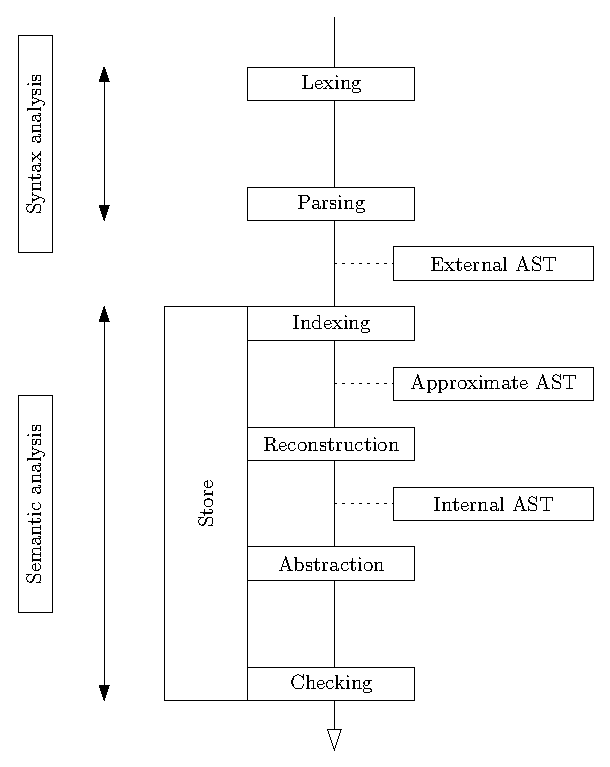
\includegraphics{figures/legacy-beluga-processing-pipeline.eps}
\caption[Overview of \Beluga version \texttt{1.0}'s processing pipeline]{%
Overview of the implementation of \Beluga version \texttt{1.0}'s processing pipeline.
The syntax analysis process converts the textual representation of \Beluga programs into an initial \acs{AST}.
The semantic analysis process refines this \acs{AST} by performing type-directed signature reconstruction, using global mutable data structures that include a store of constant declarations in the signature.
}
\label{figure:legacy-beluga-processing-pipeline}
\end{figure}

As illustrated in figure~\ref{figure:legacy-beluga-processing-pipeline}, the processing of a \Beluga signature starts with syntax analysis, which is comprised of a tokenization and parsing phase that converts the textual representation of the signature to an \ac{AST}, called the external \ac{AST}.
The model for this \ac{AST} contains ambiguous nodes, meaning that some \ac{AST} node variants capture multiple parse trees.
Specifically, the application of \LF type-level and term-level constants is represented as a list of parsemes, which effectively postpones the parsing of applications featuring user-defined operator notations.
Parsing of signature-level declarations also features auxiliary data and routines for mixing or unmixing parsemes to delegate some disambiguation to phases after context-free parsing.

Indexing in \Beluga is the process by which the concrete syntax is elaborated to a locally nameless representation called the approximate syntax, wherein bound variables are replaced with their corresponding de Bruijn indices.
As part of \Beluga's design for terse type declarations and programs, the computation of de Bruijn indices for some free variables is postponed until the abstraction phase.
Indexing is run after parsing, and is additionally responsible for disambiguating the juxtaposition of \LF parsemes at the precedence level of applications (which may contain user-defined operators), as well as disambiguating \LF types from terms and resolving constants.
This design is sensible since computing de Bruijn indices requires a stateful traversal of the \ac{AST} that accumulates lists of bindings to produce the referencing environment.
Using the centralized store of declarations, some measure of identifier overloading is supported using a pre-defined order of lookups in the referencing environment based on the kind of identifier that is expected for a given \ac{AST} node.
For instance, computation-level identifiers are resolved by looking up in order the store of computation-level variables, the store of program constants, and then the store of data type constructors.
Since names appearing in the \LF level are not part of this name resolution strategy, then an identifier can be overloaded to stand for an \LF term as well as a computation-level expression.

After indexing, the reconstruction~\cite{pientka2013insider} phase is run to reconstruct holes in types and terms, both at the \LF level and the computation level.
These holes stand for arguments omitted by the user, and provide an elegant way of abbreviating otherwise tedious aspects of programming with dependent types.
At the \LF level, approximate types are constructed to partially check the kinding of \LF types and the typing of \LF terms, as well as for guiding the synthesis of normal terms that check against a given type using typing constraints.
Type-driven unmixing of overloaded syntactic forms occurs at the meta-level, whereby meta-objects are disambiguated from substitutions during reconstruction.
The approximate \ac{AST} provides a disambiguated representation of the overall \Beluga signatures, which helps in keeping track of the various changes made during this complicated phase.

A nearly complete internal \ac{AST} as defined in figure~\ref{figure:internal-syntax} is produced at the end of reconstruction.
An abstraction phase~\cite{germain2010implementation} is run to abstract over free variables, which effectively introduces binders for implicit parameters, and unrolls the contexts of variables used during type-driven reconstruction..
This phase completes the desugaring of \Beluga programs since it finishes the computation of de Bruijn indices for variables across all levels.
The main technical challenge abstraction runs into is determining the order in which introduced binders must appear so that dependencies on terms are preserved in inferred dependent types.
This includes identifying and handling circular dependencies in abstracted parameters.

Finally, a semantic checking phase is run to ensure signature reconstruction and abstraction yielded valid programs.
This includes performing type-checking, coverage-checking and totality-checking.
These processes guarantee, respectively, that \LF-level and computation-level expressions are well-typed, that case analyses are exhaustive, and that functions annotated with a totality declaration terminate for all inputs.
Typing and coverage constraints generated during theses checking processes are statefully shared throughout this phase.
Leftover and unresolved constraints that are still in the state after having fully processed a program unit are used to signal to the user that that program is unsound within \Beluga's system.

The flow of data in the implementation of \Beluga is complex, like in most software systems.
Starting with the indexing phase, data is shared between the phases of signature reconstruction using a global mutable store.
This auxiliary data structure is a set of tables mapping constant identifiers to metadata, like in a relational database.
Crucially, the referencing environment used during indexing is computed using this store.
At any given point during the processing pipeline, the state of the store is valid since program units are processed sequentially.
New program units may be safely appended afterwards in interactive sessions.

The \Beluga system provides two ways to interactively perform queries on an existing \Beluga signature, or to augment it with new theorems.
These are the legacy \ac{REPL} and the \Harpoon system~\cite{errington2021harpoon}, the latter of which was designed as a replacement for the former.
Both systems allow the user to input \LF-level terms or computation-level expressions and get their type inferred with respect to an already elaborated \Beluga signature.
\Harpoon further enables the interactive definition and proving of theorems using sets of tactics aimed at automating proof development.
Both the \ac{REPL} and \Harpoon depend on the earlier processing phases of \Beluga and the flow of information therein.

This thesis focuses on the first few phases of the \Beluga processing pipeline, specifically parsing and indexing.
Rearchitected solutions to those phases are then shown to provide better support for some of \Beluga's and \Harpoon's existing features, while also addressing usability and soundness issues in those systems.

\section{State Management and Incremental Program Development}\label{section:intro-state-management}

Users benefit from interacting with the code they are editing by way of auxiliary software that performs actions on it.
Incremental program development in programming language tooling is the problem of applying edit actions to programs while only reprocessing a minimal portion of the program under edit.
The kinds of edit actions that can be implemented vary from one programming language to the other depending on the language's features.
Typically, edit actions include software refactoring commands such as variable renaming, reordering functions in a file, selecting a list of statements from one function and extracting them into a separate function, pretty-printing and formatting the textual representation of code, etc.
Sound and efficient handling of these edit actions is instrumental to the productivity of users working on large scale software systems.
This problem of incremental program development arises in \Beluga and \Harpoon because of the interactive tooling they provide for editing proofs, which are represented as programs.

% What is the key problem in incremental program development?

Throughout syntactic and semantic analyses pipelines, data is accumulated during the processing of any given program unit.
This data raises one of the more challenging aspects in implementing incremental program development, and the main motivation for reworking \Beluga's processing pipeline: \textit{a program unit may only be revisited with the processing state it was defined in}.
This means, for instance, that a procedure performing name lookups or mutations on an \ac{AST} at a given node may only do so using the variables and declarations in scope at that \ac{AST} node, just as the user does when editing the textual representation of that \ac{AST} node.
As such, edit actions on an \ac{AST} must preserve its semantic correctness properties so that serializing and subsequently deserializing it produces the same \ac{AST} and processing state.

% What is the preliminary step to supporting incremental program development?

A preliminary step to supporting incremental program development is to parameterize the processing routines with respect to a visitor state.
As such, those routines can be used in an out-of-order fashion as opposed to when the program is processed during compilation tasks.
This is because the routine can be visited with a different state than the one that is naturally constructed when sequentially processing program units.
For instance, a routine like conflict-avoiding variable renaming can be dependent on a referencing environment to perform variable and constant lookups.
If such a routine is invoked during an interactive program development session, then a separate routine can be implemented to rebuild the referencing environment without having to reprocess the entire program and its dependencies.
In this case, the edit action requires visiting a selected \ac{AST} node with the referencing environment as visitor state.
The issue then becomes how to efficiently construct and preserve the correctness of such visitor states.
As it pertains to \Beluga and \Harpoon, this specifically affects \ac{REPL} sessions instantiated at program holes.


\include{chapters/existing-system-architecture}

\chapter{Revised Frontend Architecture}

% TODO:

\section{Syntax Representation}

% TODO:

\section{Parser Pipeline}

% TODO:

\section{Pretty-Printing}

% What is pretty-printing?

Pretty-printing is the process that transforms an \ac{AST} back into its textual representation.
This feature of programming languages is often used to implement automated formatting software as part of tooling.
As it pertains to \Beluga and \Harpoon, pretty-printing is also used as part of debugging in order to trace the runtime execution the signature reconstruction and type-checker algorithms, as well as for displaying programmatically generated programs back to the user in interactive sessions.

% What are considerations to make when it comes to implementing pretty-printing?

Depending on the lexical conventions used during parsing, a pretty-printed \ac{AST} may not exactly correspond to its initial textual representation.
Indeed, the program's layout may change, inline comments may be printed in different locations, and extraneous parentheses may be removed.

Handling of the printed program's layout can be implemented using the algorithm described in~\cite{oppen1980prettyprinting}, whereby layout boxes and break hints are output during printing, and then actual break point locations are later computed to satisfy the layout and margin constraints.
The \OCaml standard library provides an implementation of this algorithm in its \mintinline{ocaml}|Format| module~\cite{leroy2022ocaml}.

The usual lexical convention is to treat comments as white spaces.
This simplifies the \ac{AST} representation of programs by effectively discarding all the comments.
However, during pretty-printing for formatting a program, those comments need to be restored.
A separate interval map data structure may be created during the lexing stage in order to keep track of inline comments with respect to their location.
Provided the program \ac{AST} is annotated with locations, then it is possible during printing to determine where a comment should be spliced in.

Handling of parentheses is less straightforward.
Indeed, a node in the program's \ac{AST} needs to be mapped back to the parser production that created it in order to determine its precedence.
Additionally, the associativity of operators appearing at the same precedence level must be taken into consideration to avoid producing ambiguous textual representations.

% How can pretty-printing be implemented in Beluga?

Pretty-printing of \Beluga's internal syntax requires the generation of fresh identifiers to replace de Bruijn indices.
Hence, not only is printing stateful, it also needs an auxiliary data structure containing the set of identifiers that are used by sub-expressions.
This data structure may be implement in many ways, and it reduces to the problem of annotating a tree with additional data:

\begin{itemize}
\item
Parallel data types equipped with extra fields may be defined for each kind of node in the \ac{AST}.
During pretty-printing, the \ac{AST} and this auxiliary data structure then must be traversed at the same time.
\item
Each node in the \ac{AST} may be equipped with a unique identifier to be used as key in a map data structure.
Then, lookups can be made on that map during printing to fetch the necessary data.
\item
The auxiliary data may be embedded type-safely into the \ac{AST} using recursion schemes.
\end{itemize}

The less invasive approach is to traverse the \ac{AST} in a top-down fashion and construct closures accepting the binding state to first compute the set of used offsets and then the identifiers corresponding to those offsets.

% TODO:

\section{Testing}

% TODO:


\chapter{Discussion and Conclusion}\label{chapter:conclusion}

The objectives of this thesis were to improve the design and implementation of \Beluga and \Harpoon in order fix soundness issues with the incremental development of proofs in interactive \ac{REPL} sessions.
This required revising the first few phases of syntactic and semantic analysis for the language in order to make them modular and reusable with respect to different instances of processing states.

The grammar for \Beluga and \Harpoon was fully formalized in \ac{EBNF}, along with a specification of syntactic ambiguities and how they are resolved using precedence levels and grammar blurring.
The parser was improved with the introduction of a new context-sensitive disambiguation phase.
This prevented the propagation of ambiguous \ac{AST} nodes into the more complex phases of \Beluga's processing pipeline.
By the same token, the language's was modified to support non-normal terms, which in turn allowed for syntax error messages to be improved.
The user-defined notation feature, previously limited to terms in the index language, is now fully supported at the computation-level as well.
These changes make the implementation robust, and the language more expressive and cohesive, which in turn improves the user experience.

The indexing phase was fully reimplemented using a new structure of the referencing environment at all \ac{AST} nodes in \Beluga programs and \Harpoon proof scripts.
This structure simplified the name resolution algorithm and allowed for the unification of constant declarations and indexing contexts to support simple lexical scoping rules.
In tandem, the existing implementation of namespaces for grouping signature-level declarations was rectified.
De Bruijn indices computations were implemented, and indexing for the \LF part of \Beluga was formalized to prove that the stack structure of frames can be safely leveraged to implement a checkpoint mechanism for the bindings in scope.
During \Harpoon structural editing sessions on proof scripts, the soundness of navigating between holes with respect to name resolution was rectified by ensuring that disambiguation and indexing are explicitly dependent on the referencing environment's state.

The following sections conclude this work with an evaluation of the implemented changes to \Beluga and \Harpoon, a discussion of future work to rectify long-standing issues in the later phases of semantic analysis, and finally closing remarks on the design and implementation of the system.

\section{Evaluation}

% What are the evaluation criteria for the changes?

The reimplementation of \Beluga and \Harpoon's parsing and indexing phases significantly impacted the system.
To evaluate these changes, we focus here on the non-functional requirements of runtime performance and maintainability, and then on the functional requirement of soundness.

\subsection*{Runtime Performance}

% Why was performance a concern?

Runtime performance is one of the main concerns for \Beluga and \Harpoon.
Indeed, because dependently-typed programming languages are more difficult to work with than typical languages, assisting the user with data generated during syntactic and semantic analyses is instrumental to program development.
For example, one of \Beluga's most used feature is that of displaying type information about holes in programs
Users tend to run type-checking at every step of program development to constantly refresh that information.
Consequently, in the implementation of \Beluga, a greater emphasis was placed on early error detection and reporting to minimize the latency between signature type-checking requests and the display of useful information.

% What were the impacts of the changes on performance?

Signature reconstruction has been sufficiently fast for most of the mechanizations realised in \Beluga~\texttt{v1.0}.
Consequently, the new parsing and indexing phases introduced in \texttt{v1.1} had to not degrade the runtime performance of the system.
This objective was surpassed: on a set of \num{429} test \Beluga signatures totalling approximately \num{35000} lines of code, signature reconstruction ran on average in \SI{8.412(0.133)}{\second} in \texttt{v1.0} and \SI{8.045(0.126)}{\second} in \texttt{v1.1}, which means there was a \SI{4}{\percent} runtime improvement with the revised parsing and indexing phases.
To ensure a fair comparison, these test cases were selected such that they had at most minor differences between them to mitigate the impact of breaking changes to the syntax.
The system was compiled using the same version of its dependencies, and the average of \num{15} runs was used with \num{3} warmup runs.

With an identical methodology, a similar test was carried out on a larger mechanization: with an average signature reconstruction runtime of \SI{5.504(0.024)}{\second} in \texttt{v1.0} and \SI{4.716(0.016)}{\second} in \texttt{v1.1}, there was a \SI{14}{\percent} runtime improvement.
This mechanization is mostly comprised of verbose \Harpoon proof scripts tallying over \num{90000} lines of code, which provides a better estimate for the time required to completely parse, reconstruct and type-check larger projects.
The referencing environment states at each proof hole were constructed in a separate traversal of the reconstructed \Beluga signature during the initialization of \Harpoon.
This means the soundness fixes had virtually no runtime performance impact on \Harpoon's proof navigation commands.

Although there were changes to \Beluga between \texttt{v1.0} and \texttt{v1.1} outside of the parsing, disambiguation and indexing phases, the performance improvement is best explained by the simplification of the grammar for parsing, and the usage of mutable dictionaries instead of association lists for name resolution.
Additionally, having a uniform referencing environment structure reduced the number of lookup misses that would occur when sequentially looking up declaration tables.

\subsection*{Maintainability}

% Why is maintainability a concern?

The \Beluga system has accrued significant technical debt throughout its development cycles.
This is partly explained by turnover-induced knowledge loss and lack of unit tests.
Initiatives were put in place to tackle these issues in \texttt{v1.1} during the revision of the parser.

% What were the impacts of the changes on maintainability?

To avoid turnover-induced knowledge loss, the specification for \Beluga's and \Harpoon's grammar from appendix~\ref{chapter:grammar} has been added to the code repository.
Additionally, the grammar manipulations and disambiguation mechanisms required for parsing is documented more thoroughly in the implementation.
This ensures that those steps can be repeated in the future, should the grammar be amended to support new features.

As outlined in section~\ref{section:beluga-implementation}, the parser implemented in \texttt{v1.0} returned \acp{AST} containing ambiguous nodes, and would postpone the handling of user-defined operators to the indexing phase.
This discouraged the implementation of unit tests for the parser since its outputs were incomplete and more likely to change.
In contrast, the parser revised in \texttt{v1.1} returns \acp{AST} in an unambiguous external syntax representation.
Because of this, \num{345} unit tests were added to verify the parser in isolation from the rest of the system.
These tests check success and failure scenarios for parsing small inputs for the important syntactic categories of the language and with respect to mock disambiguation states.
A unit-testing approach this precise could not have been reliably implemented in \texttt{v1.0}.
Additionally, partial round-trip testing of the parser was added for existing \Beluga examples and case studies using a pretty-printer for signatures in external syntax representation.
Complete round-trip testing is not supported since the parser discards inline comments during lexical analysis.

\subsection*{Soundness}

% Why was correctness/soundness a concern?

Throughout the development of \Beluga, a greater emphasis was placed on ensuring the soundness of it's type theory and of it's intricate semantic checks for theorem-proving.
Since this work is experimental, there are unresolved soundness issues in those later semantic checks.
To facilitate addressing them, the phases preceding those semantic checks also had to be rectified.

% What were the impacts of the changes on correctness/soundness?

Name resolution in interactive \Harpoon proof sessions was unsound in \texttt{v1.0} as explained in section~\ref{section:indexing-introduction}.
Indeed, the referencing environment was always stuck in its final state at the very end of the \Beluga signature.
This meant that out-of-order proof sessions would unsoundly have signature-level declarations brought forward in scope despite appearing at later points in the signature.
The changes introduced in \texttt{v1.1} addressed three soundness issues: fixing the handling of namespaces, allowing the shadowing of signature-level constants, and most importantly fixing the state of referencing environments when navigating to any hole in \Harpoon proof scripts.
This corrected \num{4}~test cases and generally improved the usability of both \Beluga and \Harpoon.
Top-down proof development in \Harpoon is now a viable approach for larger mechanizations.

These changes did come with trade-offs, specifically dropping the support for type-driven disambiguation of meta-level objects and for identifier overloading.
However, these additional restrictions improve the readability of \Beluga signatures since they are now simpler to disambiguate, and because identifiers refer to one declaration at a time.

\section{Future Work}

With regards to the implementation of \Beluga and \Harpoon, properly defining referencing environments and implementing indexing with respect to them is a step in the right direction.
Indeed, this allows the indexing procedures to be sound and reusable when visiting holes in \Harpoon proofs in an out-of-order fashion with respect to the \Beluga signature.
This also enables indexing to be unit-tested independently of the processing pipeline, which offers greatly visibility into the inner workings of the system, as well as provides more fine-grained verifiers of the implementation's correctness.

There are nonetheless many implementation challenges left ahead in order to fully support structural editing of \Beluga programs and \Harpoon proofs.
Indeed, there are areas of the system that still rely on the assumption that signatures are always processed in order of declaration, and hence that the signature reconstruction store only contains data about visible declarations.
The future areas of work on the implementation of \Beluga and \Harpoon include the following:

\begin{enumerate}
\item
Information flow analysis is required in the later phases of semantic analysis, namely type and term reconstruction, type-checking and unification, to ascertain whether their stateful operations are always handled soundly.
Specifically, while there is a trailing mechanism for higher-order unification to keep track of meta-variable instantiations (the assignment of a contextual object to a meta-variable), there are routines during \LF reconstruction that ignore this bookkeeping.
This can result in unsound programs when users undo edit actions during interactive proof developments.
Fixing this issue will require significant refactoring to decouple those phases from global data structures such as the signature reconstruction store.
\item
The logic proof search engine which powers \Harpoon's automation tactics uses the signature reconstruction store to have a global view of the user-defined constants and programs that can be used to solve subgoals.
As such, synthesized solutions to subgoals may reference declarations that are out of scope.
That notwithstanding, taking all constants into account during proof search may result in degraded performance and a non-responsive \ac{REPL} when using automation tactics on larger projects.
Enforcing the constraint that synthesized proofs must be sound with respect to name resolution at the holes they have to be spliced in may prune the search tree.
\item
Fresh name generation for the nameless representation of \Beluga programs is currently unsound in the implementation.
Indeed, that procedure does not wholly take into account the identifiers in scope as it restricts its focus on the declarations in indexing contexts.
This has consequences with program synthesis, both for the conversion of \Harpoon proof scripts to \Beluga programs and for error reporting.
Much like was the case with the now resolved soundness issue of navigating to holes in \Harpoon proofs, spliced \Beluga programs corresponding to \Harpoon proof scripts may refer to inadvertedly shadowed constants.
That is, a generated variable name, which is assumed to be fresh, may actually clash with a required constant name.
To address this, one needs to synthesize programs in a nameless representation and then compute readable and easily distinguishable names for variables, which effectively amounts to reversing indexing.
Dynamic programming over the tree structure of the \ac{AST} would be required to compute sets of referenced identifiers and de Bruijn indices to select appropriate names at the binding sites.
\end{enumerate}

\section{Final Remarks}

In closing, the key lessons learned from this experience with regards to programming language design and implementation are as follows:

\begin{enumerate}
\item
If a programming language is context-sensitive, separate its syntactic analysis into a context-free and a context-sensitive phase, if possible.
This ensures good runtime performance for the parser, and facilitates the integration of the language with tools that primarily support context-free languages.
\item
Keep the syntax accepted during context-free parsing simple, and rely on subsequent processing phases to disambiguate complex syntax overloading and enforce additional syntactic restrictions.
This enables error messages to be augmented with some semantic analysis to suggest corrections.
\item
Keep disambiguation and name resolution mechanisms simple and intuitive.
This ensures that programs written by users will be readable, at least at the syntactic level.
\item
Ensure that the programming language's grammar supports desugared forms for all syntactic sugars, as well as syntax for explicitly supplying what are otherwise implicit terms.
This facilitates the traceability of programs from their parsed representation to their elaborated representation, it allows users to opt out of using syntactic sugars, and it enables users to observe and verify the results of term and type reconstruction.
\item
Avoid the common programming pitfall of relying on global mutable data to capture the implemented system's state.
There will always be execution scenarios incompatible with that design, in particular incremental development, unit testing and concurrency.
\end{enumerate}


\appendix

\chapter{Disambiguation Algorithm}


\section{\acs{LF} Disambiguation}

\noindent $ \boxed{\Xi \vdash \ucorner{K} \rightsquigarrow_K K' \dashv \Xi'} $ \quad The parser object $ \ucorner{K} $ is disambiguated to the \LF kind $ K' $ under the disambiguation context $ \Xi $, which produces the output disambiguation state $ \Xi' $.

\begin{equation}
\infer{\Xi \vdash \ucorner{\mathsf{type}} \rightsquigarrow_K \mathsf{type} \dashv \Xi}{}
\end{equation}

\begin{equation}
\infer{\Xi \vdash \ucorner{A \to K} \rightsquigarrow_K A \to K \dashv \Xi}{\Xi \vdash \ucorner{A} \rightsquigarrow_A A \dashv \Xi & \Xi \vdash \ucorner{K} \rightsquigarrow_K K \dashv \Xi}
\end{equation}

\begin{equation}
\infer{\Xi \vdash \ucorner{\Pi x {:} A. K} \rightsquigarrow_K \Pi x {:} A. K \dashv \Xi}{\Xi \vdash \ucorner{A} \rightsquigarrow_A A \dashv \Xi & \Xi, x : \mathsf{LF}_{\mathsf{term}} \vdash \ucorner{K} \rightsquigarrow_K K \dashv \Xi}
\end{equation}


\noindent $ \boxed{\Xi \vdash \ucorner{A} \rightsquigarrow_A A' \dashv \Xi'} $ \quad The parser object $ \ucorner{A} $ is disambiguated to the \LF type $ A' $ under the disambiguation context $ \Xi $, which produces the output disambiguation state $ \Xi' $.

\begin{equation}
\infer{\Xi \vdash \ucorner{c} \rightsquigarrow_A c \dashv \Xi}{(c : \mathsf{LF}_{\mathsf{type}}) \in \Xi}
\end{equation}

\begin{equation}
\infer{\Xi \vdash \ucorner{A \to B} \rightsquigarrow_A A \to B \dashv \Xi}{\Xi \vdash \ucorner{A} \rightsquigarrow_A A \dashv \Xi & \Xi \vdash \ucorner{B} \rightsquigarrow_A B \dashv \Xi}
\end{equation}

\begin{equation}
\infer{\Xi \vdash \ucorner{\Pi x {:} A. B} \rightsquigarrow_A \Pi x {:} A. B \dashv \Xi}{\Xi \vdash \ucorner{A} \rightsquigarrow_A A \dashv \Xi & \Xi, x : \mathsf{LF}_{\mathsf{term}} \vdash \ucorner{B} \rightsquigarrow_A B \dashv \Xi}
\end{equation}

\begin{equation}
\infer{\Xi \vdash \ucorner{A \; M_1 \; M_2 \; \dots \; M_n} \rightsquigarrow_A A \; M_1 \; M_2 \; \dots \; M_n \dashv \Xi}{\Xi \vdash \ucorner{A} \rightsquigarrow_A A \dashv \Xi & (\Xi \vdash \ucorner{M_i} \rightsquigarrow_M M_i \dashv \Xi)_{i \in \set{1, 2, \dots, n}}}
\end{equation}


\noindent $ \boxed{\Xi \vdash \ucorner{M} \rightsquigarrow_M M' \dashv \Xi'} $ \quad The parser object $ \ucorner{M} $ is disambiguated to the \LF term $ M' $ under the disambiguation context $ \Xi $, which produces the output disambiguation state $ \Xi' $.

\begin{equation}
\infer{\Xi \vdash \ucorner{x} \rightsquigarrow_M x \dashv \Xi}{(x : \mathsf{LF}_{\mathsf{term}}) \in \Xi}
\end{equation}

\begin{equation}
\infer{\Xi \vdash \ucorner{c} \rightsquigarrow_M c \dashv \Xi}{(c : \mathsf{LF}_{\mathsf{term}}) \in \Xi}
\end{equation}

\begin{equation}
\infer{\Xi \vdash \ucorner{\lambda x {:} A. M} \rightsquigarrow_M \lambda x {:} A. M \dashv \Xi}{\Xi \vdash \ucorner{A }\rightsquigarrow_A A \dashv \Xi & \Xi, x : \mathsf{LF}_{\mathsf{term}} \vdash \ucorner{M} \rightsquigarrow M \dashv \Xi}
\end{equation}

\begin{equation}
\infer{\Xi \vdash \ucorner{M \; M_1 \; M_2 \; \dots \; M_n} \rightsquigarrow_M M \; M_1 \; M_2 \; \dots \; M_n \dashv \Xi}{\Xi \vdash \ucorner{M} \rightsquigarrow_M M \dashv \Xi & (\Xi \vdash \ucorner{M_i} \rightsquigarrow_M M_i \dashv \Xi)_{i \in \{1, 2, \dots, n\}}}
\end{equation}


\section{Contextual \acs{LF} Disambiguation}

\noindent $ \boxed{\Xi \vdash \ucorner{A} \rightsquigarrow_{A_c} A' \dashv \Xi'} $ \quad The parser object $ \ucorner{A} $ is disambiguated to the contextual \LF type $ A' $ under the disambiguation context $ \Xi $, which produces the output disambiguation state $ \Xi' $.

\begin{equation}
\infer{\Xi \vdash \ucorner{c} \rightsquigarrow_{A_c} c \dashv \Xi}{(c : \mathsf{LF}_{\mathsf{type}}) \in \Xi}
\end{equation}

\begin{equation}
\infer{\Xi \vdash \ucorner{A \to B} \rightsquigarrow_{A_c} A \to B \dashv \Xi}{\Xi \vdash \ucorner{A} \rightsquigarrow_{A_c} A \dashv \Xi & \Xi \vdash \ucorner{B} \rightsquigarrow_{A_c} B \dashv \Xi}
\end{equation}

\begin{equation}
\infer{\Xi \vdash \ucorner{\Pi x {:} A. B} \rightsquigarrow_{A_c} \Pi x {:} A. B \dashv \Xi}{\Xi \vdash \ucorner{A} \rightsquigarrow_{A_c} A \dashv \Xi & \Xi, x : \mathsf{LF}_{\mathsf{term}} \vdash \ucorner{B} \rightsquigarrow_{A_c} B \dashv \Xi}
\end{equation}

\begin{equation}
\infer{\Xi \vdash \ucorner{A \; M_1 \; M_2 \; \dots \; M_n} \rightsquigarrow_{A_c} A \; M_1 \; M_2 \; \dots \; M_n \dashv \Xi}{\Xi \vdash \ucorner{A} \rightsquigarrow_{A_c} A \dashv \Xi & (\Xi \vdash \ucorner{M_i} \rightsquigarrow_{M_c} M_i \dashv \Xi)_{i \in \{1, 2, \dots, n\}}}
\end{equation}

\begin{equation}
\infer{\Xi \vdash \ucorner{\mathsf{block} \; (x_1 : A_1, x_2 : A_2, \dots, x_n : A_n)} \rightsquigarrow_{A_c} \mathsf{block} \; (x_1 : A_1, x_2 : A_2, \dots, x_n : A_n) \dashv \Xi}{(\Xi, x_1 : \mathsf{LF}_{\mathsf{term}}, x_2 : \mathsf{LF}_{\mathsf{term}}, \dots, x_{t - 1} : \mathsf{LF}_{\mathsf{term}} \vdash \ucorner{A_t} \rightsquigarrow_{A_c} A_t \dashv \Xi)_{t \in \{1, 2, \dots, n\}}}
\end{equation}


\noindent $ \boxed{\Xi \vdash \ucorner{M} \rightsquigarrow_{M_c} M' \dashv \Xi'} $ \quad The parser object $ \ucorner{M} $ is disambiguated to the contextual \ac{LF} term $ M' $ under the disambiguation context $ \Xi $, which produces the output disambiguation state $ \Xi' $.

\begin{equation}
\infer{\Xi \vdash \ucorner{x} \rightsquigarrow_{M_c} x \dashv \Xi}{(x : \mathsf{LF}_{\mathsf{term}}) \in \Xi}
\end{equation}

\begin{equation}
\infer{\Xi \vdash \ucorner{c} \rightsquigarrow_{M_c} c \dashv \Xi}{(c : \mathsf{LF}_{\mathsf{term}}) \in \Xi}
\end{equation}

\begin{equation}
\infer{\Xi \vdash \ucorner{\lambda x {:} A. M} \rightsquigarrow_{M_c} \lambda x {:} A. M \dashv \Xi}{\Xi \vdash \ucorner{A }\rightsquigarrow_A A \dashv \Xi & \Xi, x : \mathsf{LF}_{\mathsf{term}} \vdash \ucorner{M} \rightsquigarrow M \dashv \Xi}
\end{equation}

\begin{equation}
\infer{\Xi \vdash \ucorner{M \; M_1 \; M_2 \; \dots \; M_n} \rightsquigarrow_{M_c} M \; M_1 \; M_2 \; \dots \; M_n \dashv \Xi}{\Xi \vdash \ucorner{M} \rightsquigarrow_{M_c} M \dashv \Xi & (\Xi \vdash \ucorner{M_i} \rightsquigarrow_{M_c} M_i \dashv \Xi)_{i \in \{1, 2, \dots, n\}}}
\end{equation}

% TODO: The rest


\noindent $ \boxed{\Xi; \mathbb{I}; \mathbb{P} \vdash \ucorner{M_p} \rightsquigarrow_{M_p} M_P' \dashv \Xi'; \mathbb{I}'; \mathbb{P}'} $ \quad The parser object $ \ucorner{M_p} $ is disambiguated to the contextual \LF term pattern $ M_p' $ under the outer, inner and pattern disambiguation contexts $ \Xi, \mathbb{I}, \mathbb{P} $ respectively, which produces the output outer, inner and pattern disambiguation states $ \Xi', \mathbb{I}', \mathbb{P}' $ respectively.

\begin{equation}
\infer{\Xi; \mathbb{I}; \mathbb{P} \vdash \ucorner{x} \rightsquigarrow_{M_p} x \dashv \Xi; \mathbb{I}; \mathbb{P}, x : \mathsf{LF}_{\mathsf{term}}}{x \notin \operatorname{domain}(\mathbb{I})}
\end{equation}

\begin{equation}
\infer{\Xi; \mathbb{I}; \mathbb{P} \vdash \ucorner{x} \rightsquigarrow_{M_p} x \dashv \Xi; \mathbb{I}; \mathbb{P}}{(x : \mathsf{LF}_{\mathsf{term}}) \in \Xi, \mathbb{I}}
\end{equation}

\begin{equation}
\infer{\Xi; \mathbb{I}; \mathbb{P} \vdash \ucorner{\#x} \rightsquigarrow_{M_p} \#x \dashv \Xi; \mathbb{I}; \mathbb{P}, \#x : \mathsf{LF}_{\mathsf{term}}}{\#x \notin \operatorname{domain}(\mathbb{I})}
\end{equation}

\begin{equation}
\infer{\Xi; \mathbb{I}; \mathbb{P} \vdash \ucorner{\#x} \rightsquigarrow_{M_p} \#x \dashv \Xi; \mathbb{I}; \mathbb{P}}{(\#x : \mathsf{LF}_{\mathsf{term}}) \in \Xi, \mathbb{I}}
\end{equation}

\begin{equation}
\infer{\Xi; \mathbb{I}; \mathbb{P} \vdash \ucorner{c} \rightsquigarrow_{M_p} c \dashv \Xi; \mathbb{I}; \mathbb{P}}{(c : \mathsf{LF}_{\mathsf{term}}) \in \Xi}
\end{equation}

\begin{equation}
\infer{\Xi; \mathbb{I}; \mathbb{P}^{\{0\}} \vdash \ucorner{\angled{M_1; M_2; \dots; M_n}} \rightsquigarrow_{M_p} \angled{M_1; M_2; \dots; M_n} \dashv \Xi; \mathbb{I}; \mathbb{P}^{\{n\}}}{(\Xi; \mathbb{I}; \mathbb{P}^{\{t - 1\}} \vdash \ucorner{M_t} \rightsquigarrow_{M_p} M_t \dashv \Xi; \mathbb{I}; \mathbb{P}^{\{t\}})_{t \in \{1, 2, \dots, n\}}}
\end{equation}

\begin{equation}
\infer{\Xi; \mathbb{I}; \mathbb{P} \vdash \ucorner{\lambda x {:} A. M_p} \rightsquigarrow_{M_p} \lambda x {:} A. M_p \dashv \Xi; \mathbb{I}; \mathbb{P}'}{\Xi, \mathbb{I} \vdash \ucorner{A} \rightsquigarrow_A A \dashv \Xi, \mathbb{I} & \Xi; \mathbb{I}, x : \mathsf{LF}_{\mathsf{term}}; \mathbb{P} \vdash \ucorner{M_p} \rightsquigarrow_{M_p} M_p \dashv \Xi; \mathbb{I}; \mathbb{P}'}
\end{equation}

\begin{equation}
\infer{\Xi; \mathbb{I}; \mathbb{P} \vdash \ucorner{M_p \; M_{p, 1} \; M_{p, 2} \; \dots \; M_{p, n}} \rightsquigarrow_{M_p} M_p \; M_{p, 1} \; M_{p, 2} \; \dots \; M_{p, n} \dashv \Xi; \mathbb{I}; \mathbb{P}^{\{n\}}}{\deduce{(\Xi; \mathbb{I}; \mathbb{P}^{\{t - 1\}} \vdash \ucorner{M_{p, t}} \rightsquigarrow_{M_p} M_{p, t} \dashv \Xi; \mathbb{I}; \mathbb{P}^{\{t\}})_{t \in \{1, 2, \dots, n\}}}{\Xi; \mathbb{I}; \mathbb{P} \vdash \ucorner{M_p} \rightsquigarrow_{M_p} M_p \dashv \Xi; \mathbb{I}; \mathbb{P}^{\{0\}}}}
\end{equation}

\begin{equation}
\infer{\Xi; \mathbb{I}; \mathbb{P} \vdash \ucorner{M_p : A} \rightsquigarrow_{M_p} M_p : A \dashv \Xi; \mathbb{I}; \mathbb{P}'}{\Xi, \mathbb{I} \vdash \ucorner{A} \rightsquigarrow_A A \dashv \Xi, \mathbb{I} & \Xi; \mathbb{I}; \mathbb{P} \vdash \ucorner{M_p} \rightsquigarrow_{M_p} M_p \dashv \Xi; \mathbb{I}; \mathbb{P}'}
\end{equation}

% TODO: The rest...


\section{Meta-Level Disambiguation}

\noindent $ \boxed{\Xi \vdash \ucorner{U} \rightsquigarrow_U U' \dashv \Xi'} $ \quad The parser object $ \ucorner{U} $ is disambiguated to the meta-type $ U' $ under the disambiguation context $ \Xi $, which produces the output disambiguation state $ \Xi' $.


\noindent $ \boxed{\Xi \vdash \ucorner{C} \rightsquigarrow_C C' \dashv \Xi'} $ \quad The parser object $ \ucorner{C} $ is disambiguated to the meta-object $ C' $ under the disambiguation context $ \Xi $, which produces the output disambiguation state $ \Xi' $.

\begin{equation}
\infer{\Xi \vdash \ucorner{[\Psi \vdash M_c]} \rightsquigarrow_C [\Psi \vdash M_c] \dashv \Xi}{\Xi, \Psi \vdash \ucorner{M_c} \rightsquigarrow_{M_c} M_c \dashv \Xi}
\end{equation}


\noindent $ \boxed{\Xi; \mathbb{I}; \mathbb{P} \vdash \ucorner{C_p} \rightsquigarrow_{C_p} C_p' \dashv \Xi'; \mathbb{I}'; \mathbb{P}'} $ \quad The parser object $ \ucorner{C_p} $ is disambiguated to the meta-pattern $ C_p' $ under the outer, inner and pattern disambiguation contexts $ \Xi $, $ \mathbb{I} $ and $ \mathbb{P} $, which produces the output outer, inner and pattern disambiguation contexts $ \Xi' $, $ \mathbb{I}' $ and $ \mathbb{P}' $.

\begin{equation}
\infer{\Xi; \mathbb{I}; \mathbb{P} \vdash \ucorner{[\Psi \vdash M_p] \rightsquigarrow_{C_p} [\Psi \vdash M_p]} \dashv \Xi; \mathbb{I}; \mathbb{P}'}{\Xi, \mathbb{I} \vdash \ucorner{\Psi} \rightsquigarrow_\Psi \Psi \dashv \Xi, \mathbb{I} & \Xi; \mathbb{I}, \Psi; \mathbb{P} \vdash \ucorner{M_p} \rightsquigarrow_{M_p} M_p \dashv \Xi; \mathbb{I}; \mathbb{P}'}
\end{equation}

\section{Computation-Level Disambiguation}

\noindent $ \boxed{\Xi \vdash \ucorner{\kappa} \rightsquigarrow_\kappa \kappa' \dashv \Xi'} $ \quad The parser object $ \ucorner{\kappa} $ is disambiguated to the computation-level kind $ \kappa' $ under the disambiguation state $ \Xi $, which produces the disambiguation state $ \Xi' $.

\noindent $ \boxed{\Xi \vdash \ucorner{\tau} \rightsquigarrow_\tau \tau' \dashv \Xi'} $ \quad The parser object $ \ucorner{\tau} $ is disambiguated to the computation-level type $ \tau' $ under the disambiguation state $ \Xi $, which produces the disambiguation state $ \Xi' $.

\noindent $ \boxed{\Xi \vdash \ucorner{E} \rightsquigarrow_E E' \dashv \Xi'} $ \quad The parser object $ \ucorner{E} $ is disambiguated to the computation-level expression $ E' $ under the disambiguation state $ \Xi $, which produces the disambiguation state $ \Xi' $.

\begin{equation}
\infer{\Xi \vdash \ucorner{x} \rightsquigarrow_E x \dashv \Xi}{(x : \mathsf{Comp}_{\mathsf{term}}) \in \Xi}
\end{equation}

\begin{equation}
\infer{\Xi \vdash \ucorner{c} \rightsquigarrow_E c \dashv \Xi}{(c : \mathsf{Comp}_{\mathsf{term}}) \in \Xi}
\end{equation}

\begin{equation}
\infer{\Xi \vdash \ucorner{\mathsf{fn} \; x_1 \; x_2 \; \dots \; x_n \Rightarrow E} \rightsquigarrow_E \mathsf{fn} \; x_1 \; x_2 \; \dots \; x_n \Rightarrow E \dashv \Xi}{\Xi, x_1 : \mathsf{Comp}_{\mathsf{term}}, x_2 : \mathsf{Comp}_{\mathsf{term}}, \dots, x_n : \mathsf{Comp}_{\mathsf{term}} \vdash \ucorner{E} \rightsquigarrow_E E \dashv \Xi}
\end{equation}

\begin{equation}
\infer{\Xi \vdash \ucorner{\mathsf{let} \; P = E_1 \; \mathsf{in} \; E_2} \rightsquigarrow_E \mathsf{let} \; P = E_1 \; \mathsf{in} \; E_2 \dashv \Xi}{\Xi \vdash \ucorner{E_1} \rightsquigarrow_E E_1 \dashv \Xi & \Xi; \cdot \vdash \ucorner{P} \rightsquigarrow_P P \dashv \Xi; \Xi_p & \Xi, \Xi_p \vdash \ucorner{E_2} \rightsquigarrow_E E_2 \dashv \Xi}
\end{equation}


\noindent $ \boxed{\Xi_o; \Xi_i; \Xi_p \vdash \ucorner{P} \rightsquigarrow_P P' \dashv \Xi_o'; \Xi_i'; \Xi_p'} $ \quad The parser object $ \ucorner{P} $ is disambiguated to the computation-level pattern $ P' $ under the outer, inner and pattern disambiguation states $ \Xi_o $, $ \Xi_i $ and $ \Xi_p $ respectively, which produces the output outer, inner and pattern disambiguation states $ \Xi_o' $, $ \Xi_i' $ and $ \Xi_p' $ respectively.

\begin{equation}
\infer{\Xi_o; \Xi_i; \Xi_p \vdash \ucorner{\{ x : g \} P} \rightsquigarrow_P \{ x : g \} P \dashv \Xi_o; \Xi_i; \Xi_p'}{\deduce{\Xi_o; \Xi_i, x : \mathsf{Ctx}; \Xi_p, x : \mathsf{Ctx} \vdash \ucorner{P} \rightsquigarrow_P P \dashv \Xi_o; \Xi_i; \Xi_p'}{(g : \mathsf{Schema}) \in \Xi_o, \Xi_i & x \notin \Domain(\Xi_p)}}
\end{equation}


\section{\Harpoon Disambiguation}

\section{\Beluga Signature Disambiguation}

\noindent $ \boxed{\Xi; \mathbb{M} \vdash \ucorner{D} \rightsquigarrow_D D' \dashv \Xi'; \mathbb{M}'} $ \quad The parser object $ \ucorner{D} $ is disambiguated to the \Beluga signature declaration $ D' $ under the outer and module disambiguation contexts $ \Xi $ and $ \mathbb{M} $ respectively, which produces the output outer and module disambiguation states $ \Xi' $ and $ \mathbb{M}' $ respectively.

\begin{equation}
\infer{
	\splitdfrac{
		\Xi; \mathbb{M} \vdash \ucorner{\mathsf{module} \; x = \mathsf{struct} \; D_1 \; D_2 \; \dots \; D_n \; \mathsf{end}} \rightsquigarrow_D
	}{
		\splitdfrac{
			\mathsf{module} \; x = \mathsf{struct} \; D_1 \; D_2 \; \dots \; D_n \; \mathsf{end} \dashv
		}{
			\Xi, x : \mathsf{module}(\mathbb{M}^{\{n\}}); \mathbb{M}, x : \mathsf{module}(\mathbb{M}^{\{n\}})
		}
	}
}{
	\deduce{(\Xi^{\{t - 1\}}; \mathbb{M}^{\{t - 1\}} \vdash \ucorner{D_t} \rightsquigarrow_D D_t \dashv \Xi^{\{t\}}; \mathbb{M}^{\{t\}})_{t \in \{1, 2, \dots, n\}}}{\Xi^{\{0\}} = \Xi & \mathbb{M}^{\{0\}} = \cdot}
}
\end{equation}

\begin{equation}
\infer{
	\Xi; \mathbb{M} \vdash \ucorner{\mathsf{\text{-}\text{-}open} \; c.} \rightsquigarrow_D \mathsf{\text{-}\text{-}open} \; c. \dashv \Xi, \Xi_c; \mathbb{M}
}{
	(c : \mathsf{module}(\Xi_c)) \in \Xi
}
\end{equation}

\begin{equation}
\infer{
	\Xi; \mathbb{M} \vdash \ucorner{x : K} \rightsquigarrow_D x : K \dashv \Xi, x : \mathsf{LF}_{\mathsf{type}}; \mathbb{M}, x : \mathsf{LF}_{\mathsf{type}}
}{
	\Xi \vdash \ucorner{K} \rightsquigarrow_K K \dashv \Xi
}
\end{equation}

\begin{equation}
\infer{
	\Xi; \mathbb{M} \vdash \ucorner{x : A} \rightsquigarrow_D x : A \dashv \Xi, x : \mathsf{LF}_{\mathsf{term}}; \mathbb{M}, x : \mathsf{LF}_{\mathsf{term}}
}{
	\Xi \vdash \ucorner{A} \rightsquigarrow_A A \dashv \Xi
}
\end{equation}

\begin{equation}
\infer{
	\splitdfrac{
		\Xi; \mathbb{M} \vdash \ucorner{\mathsf{LF} \; x : K = x_1 : A_1 \mid x_2 : A_2 \mid \dots \mid x_n : A_n;} \rightsquigarrow_D
	}{
		\splitdfrac{
			\mathsf{LF} \; x : K = x_1 : A_1 \mid x_2 : A_2 \mid \dots \mid x_n : A_n; \dashv
		}{
			\Xi, x : \mathsf{LF}_{\mathsf{type}}, (x_t : \mathsf{LF}_{\mathsf{term}})_{t \in \{1, 2, \dots, n\}}; \mathbb{M}, x : \mathsf{LF}_{\mathsf{type}}, (x_t : \mathsf{LF}_{\mathsf{term}})_{t \in \{1, 2, \dots, n\}}
		}
	}
}{
	\deduce{
		(\Xi, x : \mathsf{LF}_{\mathsf{type}} \vdash \ucorner{A_t} \rightsquigarrow_A A_t \dashv \Xi, x : \mathsf{LF}_{\mathsf{type}})_{t \in \{1, 2, \dots, n\}}
	}{
		\Xi \vdash \ucorner{K} \rightsquigarrow_K K \dashv \Xi
	}
}
\end{equation}



\bibliographystyle{plain}

\bibliography{bibliography}

\end{document}
